%!Tex Root = ../main.tex
% ./Packete.tex
% ./Design.tex
% ./Deklarationen.tex
% ./Vorbereitung.tex
% ./Aufgabe1.tex
% ./Aufgabe2.tex
% ./Aufgabe3.tex
% ./Aufgabe4.tex

\section{Bonus}

\begin{frame}[allowframebreaks]{Bonus}{Vollständige Induktion über natürliche Zahlen\vspace{0.5cm}}
  \begin{itemize}
    \item für \alert{Allbehauptungen}: $\forall n\in\mathbb{N}:\mathcal{E}(n)$ (Eigenschaft $\mathcal{E}$)
    \item die allgemeine Form wird als \alert{Strukturelle Induktion} bezeichnet, \alert{Vollständige Induktion} ist zum Beweis von Aussagen für alle Natürlichen Zahlen
    \begin{itemize}
      \item Menge der \alert{natürlichen Zahlen} $\mathbb{N}$ weißt geignete Struktur auf, da auf ihnen die Nachfolgerbeziehung besteht
    \end{itemize}
    \item man führt Teilbewise für $2$ Fälle: 
    \begin{itemize}
      \item \alert{Basisfall:} ${\mathcal{E}}(0)$, d.h. die natürliche Zahl $0$ hat die Eigenschaft $\epsilon$
      \item \alert{Induktionsfall:} $\forall i\in\mathbb{N} \left(\mathcal{E}(i)\Rightarrow\mathcal{E}(i+1)\right)$, d.h. die Eigenschaft $\epsilon$ überträgt sich von jeder natürlichen Zahl $i$ auf ihren Nachfolger $i + 1$
    \end{itemize}
    \item bei beweisender Allbehauptung für den Induktionsfall wird Implikation: Sei $i\in\mathbb{N}$ beliebig. Zu zeigen: $\epsilon(i)\Rightarrow\epsilon(i+1)$ zerlegt in: Sei $i\in\mathbb{N}$ beliebig. Es gelte: $\epsilon(i)$. Zu zeigen: $\epsilon(i+1)$
    \item Diese Darstellung des Induktionsfalls legt seine Zerlegung in die üblichen drei Bestandteile \alert{Induktionsannahme}, \alert{Induktionsbehauptung}, \alert{Induktionsschritt} nahe:
  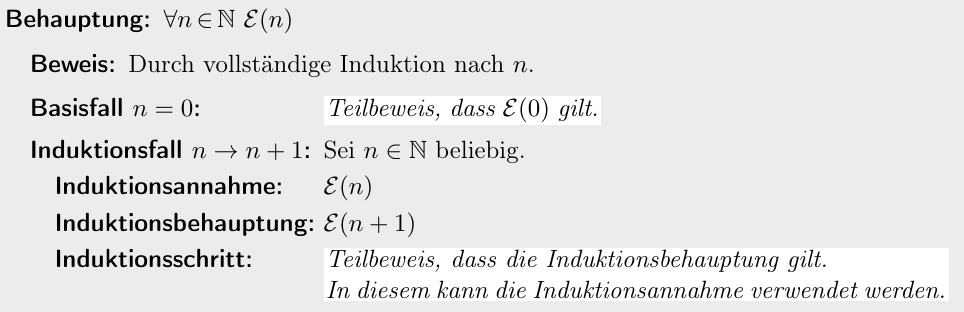
\includegraphics[width=\linewidth]{./figures/vollstaendige_induktion.png}
  \end{itemize}
  \begin{itemize}
    \item Induktionsfall beweist Allbehauptung mit darin enthaltener Implikationsbehauptung 
    \item Wenn für Eigenschaft $\epsilon$ Basisfall und Induktionsfall bewiesen sind, gilt, dass jede natürliche Zahl die Eigenschaft $\epsilon$ hat, denn:
    \begin{enumerate}
      \setcounter{enumi}{-1}
      \item Wegen des Basisfalls gilt $\epsilon(0)$.
      \item Mit $\epsilon(0)$ gilt wegen des Induktionsfalls auch $\epsilon(1)$.
      \item Mit $\epsilon(1)$ gilt wegen des Induktionsfalls auch $\epsilon(2)$.
      \item Mit $\epsilon(2)$ gilt wegen des Induktionsfalls auch $\epsilon(3)$.
      \item $\ldots$
    \end{enumerate}
  \end{itemize}
  \includegraphics[width=0.6\textwidth]{./figures/vollständige_induktion_1.png}
  \includegraphics[width=0.8\textwidth]{./figures/vollständige_induktion_2.png}
\end{frame}

\begin{frame}[allowframebreaks]{Bonus}{O-Notation}
  \begin{itemize}
    \item Man will Funktionen irendwie vergleichen und das einzige sinnvolle was man vergleichen kann ist die \alert{Wachstumsrate}, denn für zwei Funktionen kann gleichzeitig gelten: $g = O(f)$, also $g$ wächst nicht stärker als $f$ und $g > f$, also $g$ ist überall echt größer als $f$
    \item Konstate Faktoren und Summanden $c \cdot x$ und $c + x$ sollen keine Rolle, aber es geht um \alert{Wachstumsrate}, Konstante Faktoren und Summanden spielen keine Rolle
    \item Die Operatoren $O, \Omega, \Theta, o, \omega$ sind auf Funktionen, was die Operatoren $\le, \ge, =, <, >$ auf Zahlen sind
    \item man sagt die \enquote{Laufzeit eines Algorihmus ist: $\Omega(n\cdot log(n))$}, man sagt \alert{NICHT}, dass ein \enquote{Algorithmus Laufzeit mindestens $O(n\cdot log(n))$ hat}
    \item \alert{formal:} 
    \begin{itemize}
      \item $O(f)= \{g: \mathbb{N}\to\mathbb{R} | \exists n_0\in\mathbb{N}, \exists C > 0, \forall n\ge n_0, g(n)\le C \cdot f(n)\}$
      \item $\Omega(f)= \{g: \mathbb{N}\to\mathbb{R} | \exists n_0\in\mathbb{N}, \exists C > 0, \forall n\ge n_0, g(n)\ge C \cdot f(n)\}$
      \item $o(f)= \{g: \mathbb{N}\to\mathbb{R} | \exists n_0\in\mathbb{N}, \exists C > 0, \forall n\ge n_0, g(n)\ge C \cdot f(n)\}$
      \item $\omega(f)= \{g: \mathbb{N}\to\mathbb{R} | \exists n_0\in\mathbb{N}, \exists C > 0, \forall n\ge n_0, g(n)\ge C \cdot f(n)\}$
    \end{itemize}
    \item \alert{Bestimmung über Grenzwerte:}
    \begin{enumerate}
      \item $\displaystyle f=O(g) \Leftrightarrow \operatorname{lim}_{n\to\infty}\frac{f(n)}{g(n)} < \infty$
      \item $\displaystyle f=\Omega(g) \Leftrightarrow \operatorname{lim}_{n\to\infty}\frac{f(n)}{g(n)} > 0$
      \item $\displaystyle f=\Theta(g) \Leftrightarrow \operatorname{lim}_{n\to\infty}\frac{f(n)}{g(n)} > 0$ und $\displaystyle\operatorname{lim}_{n\to\infty}\frac{f(n)}{g(n)} < \infty$
      \item $\displaystyle f=o(g) \Leftrightarrow \operatorname{lim}_{n\to\infty}\frac{f(n)}{g(n)} = 0$
      \item $\displaystyle f=\omega(g) \Leftrightarrow \operatorname{lim}_{n\to\infty}\frac{f(n)}{g(n)} = \infty$
    \end{enumerate}
  \end{itemize}
\end{frame}

\begin{frame}{Bonus}{Regel von L'Hopital}
  \begin{itemize}
    \item $\displaystyle \operatorname*{lim}_{x\to c}{\frac{f(x)}{g(x)}}=\operatorname*{lim}_{x\to c}{\frac{f^{\prime}(x)}{g^{\prime}(x)}}$
    \begin{itemize}
      \item wird verwendet bei Grenzwertbetrachtung bei der man bei Zähler und Nenner entweder den Fall $\frac{0}{0}$ oder $\frac{\pm\infty}{\pm\infty}$ hat und beide Ableitungen differenzierbar % und $g(x)\ne 0$ für $x\ne y$ für den Fall $\frac{0}{0}$ und $g(x)'\ne 0$ für den Fall $\frac{\infty}{\infty}$ 
      \item dann Zähler und Nenner des Bruches getrennt voneinander ableiten und dann nochmal Grenwertbetrachtung
      \item wenn nochmal unbestimmter Ausdruck rauskommt und wieder entweder der Fall $\frac{0}{0}$ oder $\frac{\infty}{\infty}$ und beide Ableitungen differenzierbar, dann nochmal anwenden oder sonst Pech gehabt
    \end{itemize}
  \end{itemize}
\end{frame}
